\chapter{Screen Registry and Recipe Model}
\label{ch:registry-and-recipes}

\section{Concept}

The registry is a catalogue of \emph{screen recipes}. A recipe is pure data: it
declares what a screen is called, which stacks it supports, which npm packages it
needs, and which files it produces. Files are produced by rendering Handlebars
templates, and a recipe may define multiple entries for the same output path, each
guarded by a \texttt{when} condition, so that one recipe yields stack-specific
output.

\section{Recipe schema}

The schema is defined in \texttt{packages/registry/schema.json} (JSON Schema
Draft-07) and mirrored by the TypeScript interface in
\texttt{packages/core/src/types.ts}.

\begin{longtable}{@{}L{2.7cm}L{2.1cm}L{2cm}L{7.2cm}@{}}
\caption{Recipe fields}\\
\toprule
\textbf{Field} & \textbf{Type} & \textbf{Required} & \textbf{Description} \\
\midrule
\endfirsthead
\toprule
\textbf{Field} & \textbf{Type} & \textbf{Required} & \textbf{Description} \\
\midrule
\endhead
\texttt{id} & string & yes & Pattern \texttt{\^{}[a-z0-9-]+/[a-z0-9-]+\$}; must equal the
file path relative to \texttt{data/} without the extension. \\
\texttt{name} & string & yes & Human-readable name, min length 3. \\
\texttt{description} & string & yes & Short description, min length 10. \\
\texttt{version} & string & yes & Semver pattern \texttt{\^{}\textbackslash d+\textbackslash.\textbackslash d+\textbackslash.\textbackslash d+\$}. \\
\texttt{framework} & enum & yes & Only \texttt{"react-native"}. \\
\texttt{runtime} & enum & yes & Only \texttt{"expo"}. \\
\texttt{typescript} & boolean & no & Whether the recipe is authored TypeScript-first. \\
\texttt{supported} & object & yes & Four option arrays: styling, router, ui, icons. \\
\texttt{dependencies} & string[] & yes & npm packages installed with \texttt{add}. \\
\texttt{devDependencies} & string[] & no & npm packages installed with \texttt{add -D}. \\
\texttt{files} & array & yes & File entries (see below), min 1 item. \\
\texttt{variants} & array & no & Named variants, each \texttt{\{id, label, description?\}}. \\
\texttt{tags} & string[] & no & Search keywords. \\
\texttt{primitives} & string[] & no & Primitive recipe ids required when
\texttt{ui === "shadcn"}. \\
\bottomrule
\end{longtable}

\subsection*{File entry}

\begin{longtable}{@{}L{2.7cm}L{11.1cm}@{}}
\caption{File entry fields}\\
\toprule
\textbf{Field} & \textbf{Meaning} \\
\midrule
\endfirsthead
\toprule
\textbf{Field} & \textbf{Meaning} \\
\midrule
\endhead
\texttt{path} & Output path relative to the project root. \\
\texttt{template} & Inline Handlebars template string (used at render time). \\
\texttt{templateFile} & Path to a \texttt{.hbs} file, relative to
\texttt{packages/registry/templates}; inlined into \texttt{template} at build
time and the field is deleted from the emitted recipe. \\
\texttt{perStyling} & Map from styling option to a template string or \texttt{.hbs}
path (inlined at build time). \\
\texttt{when} & Condition object with optional \texttt{styling}, \texttt{router},
\texttt{ui}, \texttt{icons} arrays and \texttt{typescript} boolean. \\
\texttt{variants} & Map from variant id to a template string or \texttt{.hbs} path
(inlined at build time). \\
\bottomrule
\end{longtable}

\subsection*{Enumerations}

\begin{table}[H]
\centering
\caption{Option enumerations (from the schema and the core types)}
\begin{tabular}{@{}L{3cm}L{10.8cm}@{}}
\toprule
\textbf{Option} & \textbf{Allowed values} \\
\midrule
styling & \texttt{nativewind}, \texttt{stylesheet}, \texttt{tamagui} \\
router & \texttt{expo-router}, \texttt{react-navigation} \\
ui & \texttt{native}, \texttt{shadcn}, \texttt{custom} \\
icons & \texttt{lucide}, \texttt{vector-icons}, \texttt{none} \\
\bottomrule
\end{tabular}
\end{table}

\textbf{Implementation gap.} \texttt{tamagui}, \texttt{vector-icons} and
\texttt{custom} are legal per the schema and the type unions, and are offered in VS
Code settings, but \emph{no recipe declares them}, and the CLI prompt lists only
\texttt{nativewind}/\texttt{stylesheet} and \texttt{lucide}/\texttt{none}. See
Chapter~\ref{ch:known-issues}.

\section{Catalog statistics}

\begin{table}[H]
\centering
\caption{Catalog composition (verified)}
\begin{longtable}{@{}L{3.2cm}L{1.6cm}L{9cm}@{}}
\toprule
\textbf{Category} & \textbf{Recipes} & \textbf{Ids} \\
\midrule
\endhead
app & 5 & \texttt{app/home}, \texttt{app/notifications}, \texttt{app/profile},
\texttt{app/search}, \texttt{app/settings} \\
auth & 4 & \texttt{auth/login}, \texttt{auth/register},
\texttt{auth/forgot-password}, \texttt{auth/otp-verification} \\
calendar & 1 & \texttt{calendar/schedule} \\
chat & 1 & \texttt{chat/conversations} \\
content & 1 & \texttt{content/article-reader} \\
dashboard & 1 & \texttt{dashboard/analytics} \\
ecommerce & 2 & \texttt{ecommerce/products}, \texttt{ecommerce/product-details} \\
map & 1 & \texttt{map/location} \\
onboarding & 3 & \texttt{onboarding/welcome}, \texttt{onboarding/features},
\texttt{onboarding/permissions} \\
ui & 3 & \texttt{ui/button}, \texttt{ui/input}, \texttt{ui/utils} \\
utility & 2 & \texttt{utility/empty}, \texttt{utility/error} \\
\midrule
\textbf{Total} & \textbf{24} & --- \\
\bottomrule
\end{longtable}
\end{table}

Templates: \textbf{48} \texttt{.hbs} files under
\texttt{packages/registry/templates}, organised by the same category structure.

\section{Variants}

Only three recipes declare a variant, all with the id \texttt{glass} and label
``Glassmorphism'':
\texttt{app/home} (\texttt{app.home.index.glass.hbs}),
\texttt{auth/login} (\texttt{app.login.index.glass.hbs}) and
\texttt{onboarding/welcome} (\texttt{app.welcome.index.glass.hbs}).

The remaining twenty-one recipes declare \texttt{"variants": []}.

The glass templates render a dark surface (\texttt{\#0F172A}) with translucent
overlays (\texttt{rgba(255,255,255,0.08)}) and, for \texttt{auth/login}, import
\texttt{BlurView} from \texttt{expo-blur}; note that \texttt{expo-blur} is not
declared in that recipe's \texttt{dependencies} array (see
Chapter~\ref{ch:known-issues}).

\section{Template organisation}

\begin{lstlisting}[language=bash]
packages/registry/templates/
  app/home/app.home.index.hbs
  app/home/app.home.index.glass.hbs
  auth/login/app.login.index.hbs
  auth/login/app.login.index.shadcn.hbs
  auth/login/app.login.index.glass.hbs
  auth/login/components.login-form.hbs
  auth/login/components.login-form.shadcn.hbs
  auth/login/screens.loginscreen.react-navigation.hbs
  auth/login/hooks.use-login.hbs
  ui/button.hbs
  ui/input.hbs
  ui/lib.utils.hbs
  ...
\end{lstlisting}

The naming convention is \texttt{<path-with-dots>.<variant-suffix>.hbs}, for
example \texttt{components.login-form.shadcn.hbs} for the shadcn variant of
\texttt{components/LoginForm.tsx}.

\section{Build and distribution}

\begin{figure}[H]
\centering
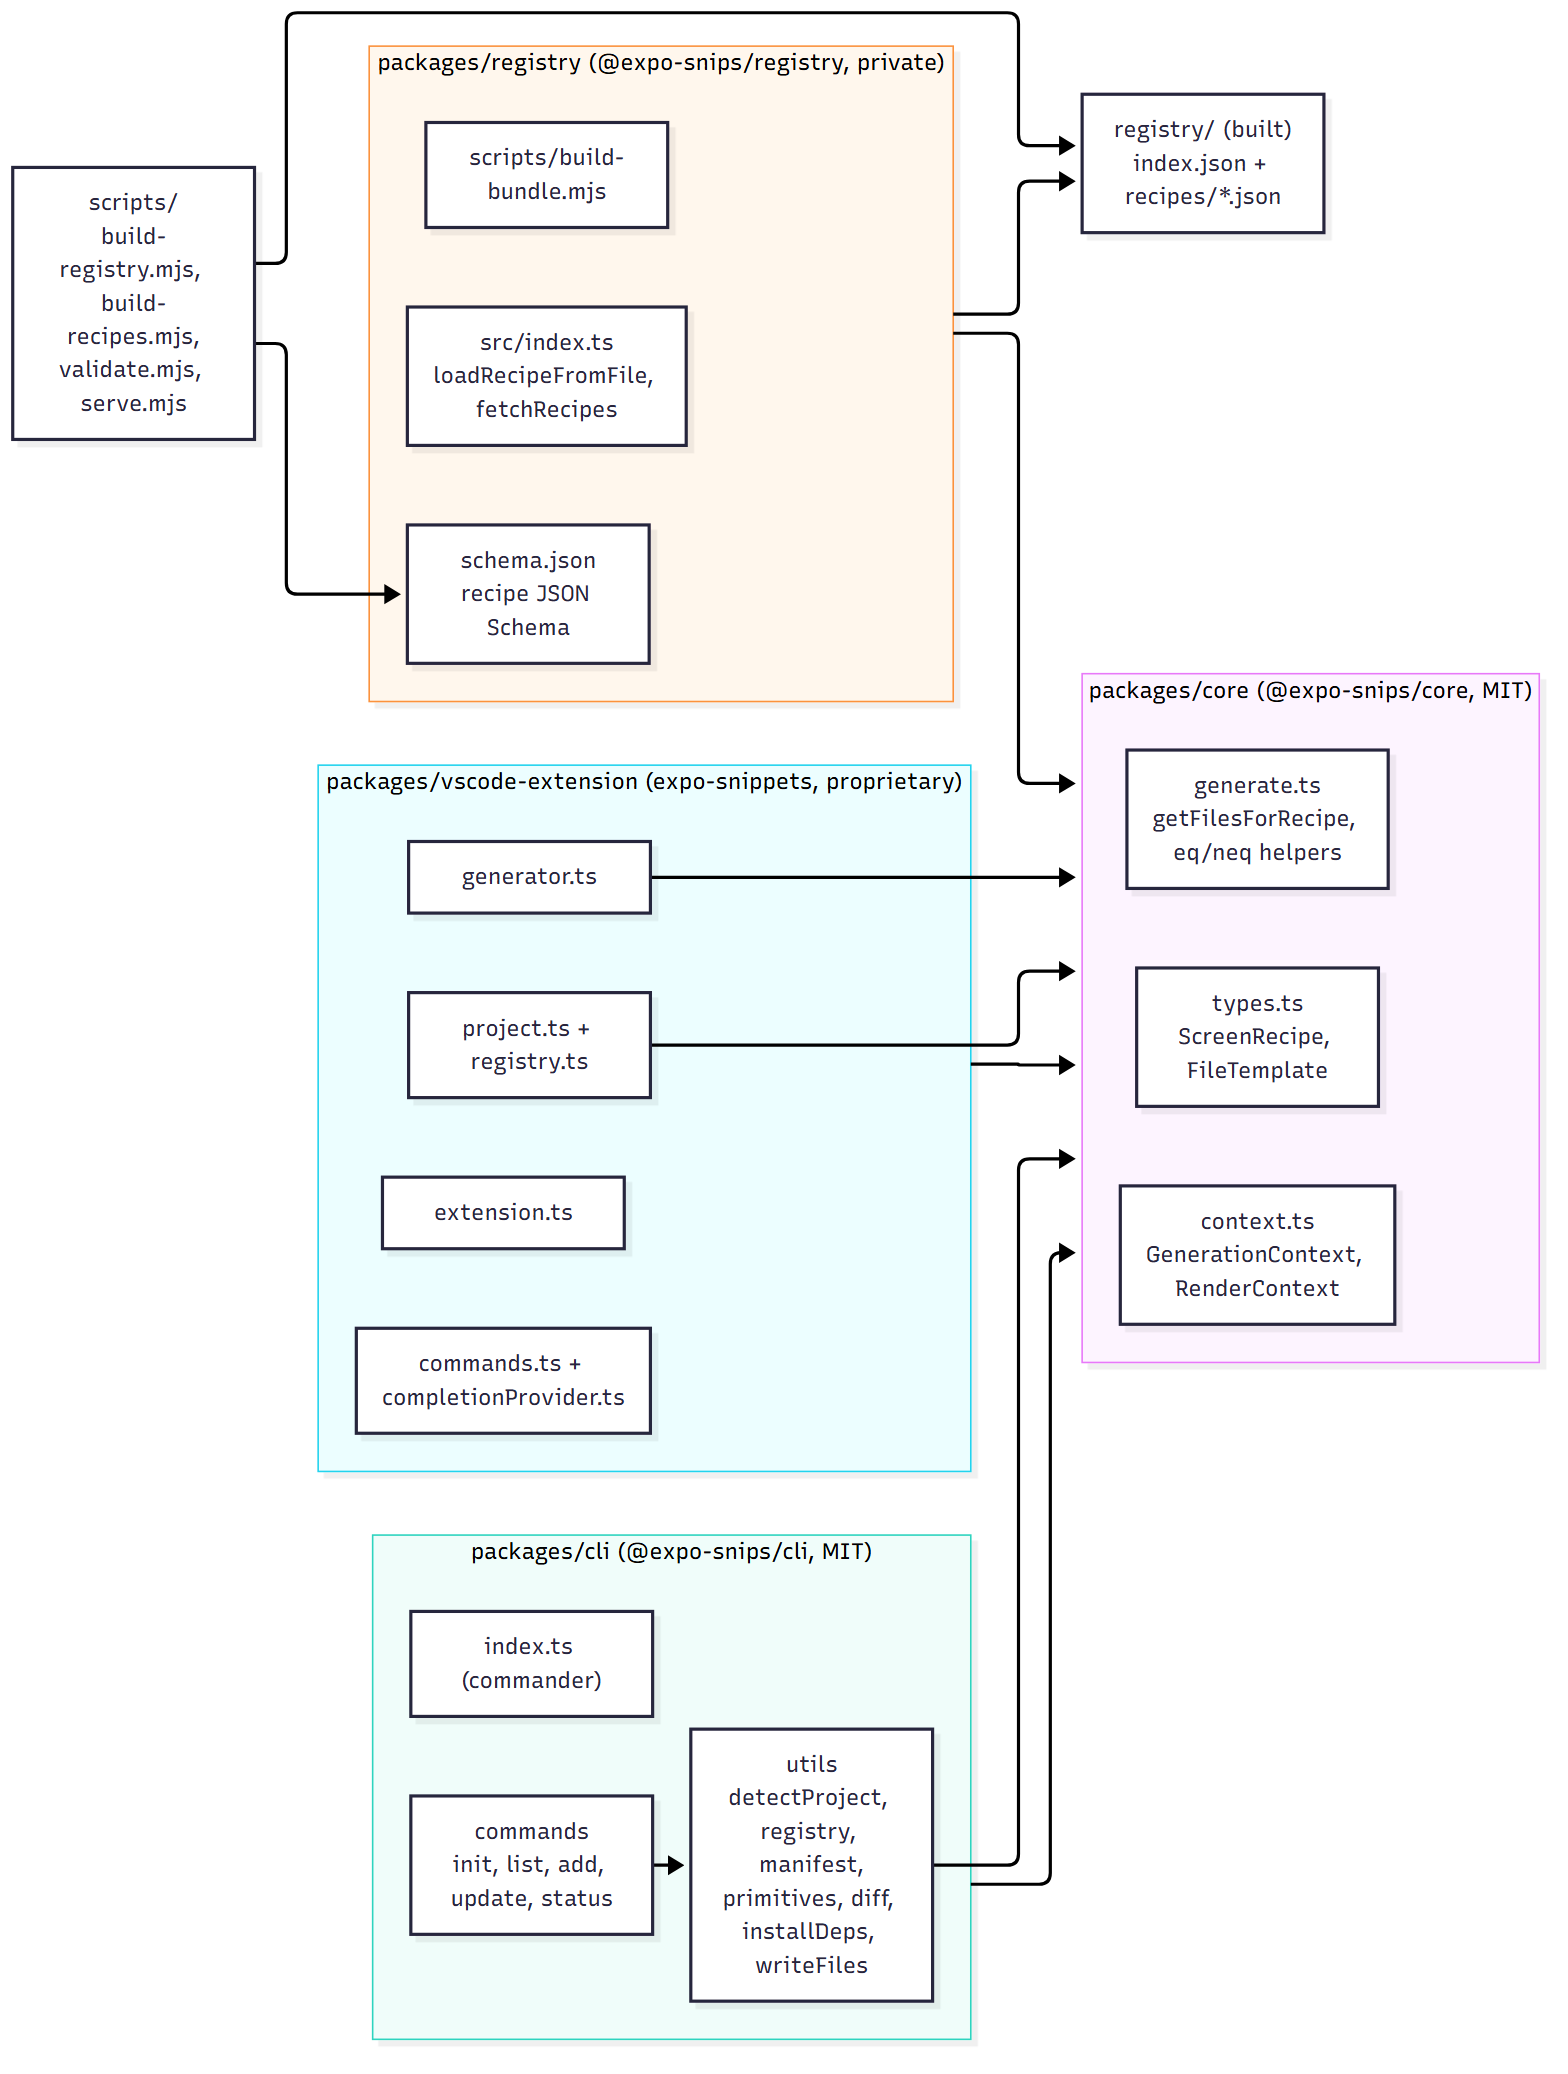
\includegraphics[width=0.98\textwidth]{diagrams/component-architecture.png}
\caption{Recipe data flows into the built registry and into the embedded client bundles}
\label{fig:registry-build}
\end{figure}

\begin{longtable}{@{}L{4.6cm}L{9.4cm}@{}}
\caption{Build outputs derived from the recipe sources}\\
\toprule
\textbf{Output} & \textbf{Producer and purpose} \\
\midrule
\endfirsthead
\toprule
\textbf{Output} & \textbf{Producer and purpose} \\
\midrule
\endhead
\texttt{registry/index.json} & \texttt{scripts/build-registry.mjs}. Index entries for
all 24 recipes; served at \texttt{\{base\}/index.json}. \\
\texttt{registry/recipes/<id>.json} & \texttt{scripts/build-registry.mjs}. Full
recipes with inlined templates; served at \texttt{\{base\}/recipes/<id>.json}. \\
\texttt{packages/registry/bundle.json} & \texttt{scripts/build-bundle.mjs}. A
\texttt{\{version:1, name, recipes\}} bundle for offline consumption. \\
\texttt{packages/cli/src/generated/registry-data.ts} & \texttt{scripts/prepare-registry.mjs}.
Embedded catalog for the CLI. \\
\texttt{packages/vscode-extension/src/generated/registry-data.ts} & Same script;
embedded catalog for the extension. \\
\bottomrule
\end{longtable}

All four derived outputs are produced from the single source of truth in
\texttt{packages/registry/data} and \texttt{packages/registry/templates}. The
generated per-client modules are git-ignored
(\texttt{.gitignore}, lines 7--8). The built \texttt{registry/} folder is committed
and is rebuilt (deleted first) by the build script.

\section{Validation}

\texttt{scripts/validate.mjs} (run with \texttt{pnpm validate}) implements a
hand-written subset of JSON Schema Draft-07 validation. For each file under
\texttt{data/} it checks:

\begin{itemize}
  \item all required fields are present;
  \item \texttt{id} matches \texttt{\^{}[a-z0-9-]+/[a-z0-9-]+\$};
  \item \texttt{version} matches the three-part semver pattern;
  \item \texttt{framework} is \texttt{react-native} and \texttt{runtime} is
        \texttt{expo};
  \item every \texttt{supported.*} value is a legal enum member;
  \item \texttt{files} is a non-empty array and every entry has both \texttt{path}
        and \texttt{templateFile};
  \item \texttt{id} equals the file's path relative to \texttt{data/};
  \item every referenced template file exists on disk.
\end{itemize}

It prints a per-recipe pass/fail line and exits non-zero when any error is found.
It is the only automated verification in the repository.

\textbf{Note.} Because the emitted recipes replace \texttt{templateFile} with
\texttt{template}, validation must run against the \emph{source} data directory;
the validator is invoked by \texttt{pnpm validate} precisely for that reason.
